\documentclass[aspectratio=169]{beamer}

\usepackage{amsmath,amssymb}
\usepackage{booktabs}
\usepackage{tabularx}
\usepackage{tikz}
\usetikzlibrary{arrows.meta,calc,positioning,shapes.geometric}
\usepackage[main=vietnamese,english]{babel}
\usepackage{graphicx}
\graphicspath{{assets/}{../PA2/img/mvp/}}
\usepackage{ragged2e}
\usepackage{csquotes}
\usepackage[backend=biber,style=authoryear,maxcitenames=2,doi=false,isbn=false,url=true]{biblatex}
\addbibresource{refs.bib}

\definecolor{mutuxBlue}{HTML}{356AE6}
\definecolor{mutuxTeal}{HTML}{00A6A6}
\definecolor{mutuxOrange}{HTML}{F08A4B}

\usetheme[
  accent=mutuxBlue,
  progressbar=foot,
  sectionpage=none,
  numbering=fraction,
  numberrail=subsection,
  block=fill,
  notes=hide,
  toc=none,
  closing=none
]{cookie}
\lstset{style=cookie}

\title[Mutux]{Mutux}
\subtitle{Thuê thử gaming gear trước khi mua}
\author[Startup K23]{Nhóm Mutux}
\cookieemail{mutux.startup@gmail.com}
\institute{Đồ án Khởi nghiệp K23 -- Khoa Công nghệ Thông tin}
\cookieuni{Trường Đại học Khoa học Tự nhiên -- ĐHQG-HCM}
\cookielocation{Thành phố Hồ Chí Minh}
\date{2026}
\cookietagline{Gear Up. Play On.}
\cookieclosingtitle{Cùng Mutux biến trải nghiệm thành quyết định đúng}
\cookieclosingtext{Thuê thử gear chuẩn gu, mua khi đã chắc.}
\cookieclosingqr{https://github.com/}
\cookieclosingqrlabel{Prototype và mã nguồn dự án}

\titlegraphic{%
  \begin{tikzpicture}[scale=.72]
    \fill[white,opacity=.94] (0,0) circle[radius=1.15];
    \foreach \x/\y/\r in {-.43/.40/.12,.36/.50/.10,.52/-.22/.13,-.38/-.43/.09,.02/.02/.11}
      \fill[mutuxBlue!82!black] (\x,\y) circle[radius=\r];
  \end{tikzpicture}%
}

\newcommand{\metric}[2]{%
  \begin{minipage}[t]{.22\textwidth}\centering
    {\color{mutuxBlue}\fontsize{23}{25}\selectfont\bfseries #1}\par
    \vspace{.15em}\scriptsize #2
  \end{minipage}%
}

\begin{document}
\maketitle

\section{Vấn đề}

\begin{frame}{Vấn đề nhóm đang giải quyết}{Người dùng phải mua trước khi biết gaming gear có hợp mình hay không}
  \vspace{.6em}
  \begin{columns}[T,onlytextwidth]
    \column{.30\textwidth}
      \cookiekicker{Giá trị thử sai lớn}\par\vspace{.45em}
      Gear tốt thường có giá vài triệu đồng cho mỗi lần thử.
    \column{.30\textwidth}
      \cookiekicker{Thông tin chưa đủ}\par\vspace{.45em}
      Review và thông số chỉ cho biết sản phẩm ``tốt trên giấy''.
    \column{.30\textwidth}
      \cookiekicker{Trải nghiệm quá ngắn}\par\vspace{.45em}
      Showroom không phản ánh cảm giác dùng lâu dài.
  \end{columns}
  \vfill
  \centering\textcolor{mutuxOrange}{\textbf{Người dùng ra quyết định trong trạng thái thiếu chắc chắn.}}
\end{frame}

\begin{frame}{Hệ quả của việc mua khi chưa chắc}{Chi phí thử sai rơi hết về phía người dùng}
  \vspace{.4em}
  \centering
  \begin{tikzpicture}[node distance=9mm]
    \node[cookie accent node,minimum width=2.6cm] (a) {Mua nhầm};
    \node[cookie node,minimum width=2.6cm,right=of a] (b) {Tốn tiền};
    \node[cookie node,minimum width=2.9cm,right=of b] (c) {Khó bán lại};
    \foreach \x/\y in {a/b,b/c} \draw[cookie arrow] (\x) -- (\y);
  \end{tikzpicture}
  \vfill
  \begin{alertblock}{Khoảng trống hiện tại}
    Chưa có cách nào để dùng thử gear đủ lâu, trong chính không gian chơi của mình, trước khi xuống tiền.
  \end{alertblock}
\end{frame}

\section{Cơ hội khởi nghiệp}

\begin{frame}{Esports Việt Nam bước vào giai đoạn chuyên nghiệp hóa}{Lễ ký kết chiến lược 2026--2030 là tín hiệu cho một hệ sinh thái đang mở rộng}
  \begin{columns}[c,onlytextwidth]
    \column{.48\textwidth}
      
\includegraphics[width=\linewidth,height=.56\textheight,keepaspectratio]{clavis-esport-inline-1.jpg}\par
      \vspace{.3em}
      {\centering\scriptsize\color{cookieMuted}
      Lễ ký kết chiến lược phát triển Esports quốc gia 2026--2030, ngày 14/5/2026.\par}
    \column{.43\textwidth}
      \cookiekicker{TÍN HIỆU THỊ TRƯỜNG}\par\vspace{.45em}
      \begin{itemize}
        \item Chiến lược được ký kết ngày 14/5/2026.
        \item Hệ sinh thái được định hướng phát triển qua công nghệ, giải đấu, doanh nghiệp và cộng đồng.
      \end{itemize}
  \end{columns}
  \note{[Sources]
    Nội dung và ảnh: Ngô Võ Quốc Vương, ``Esport là gì? Vì sao Esport đang trở thành ngành kinh tế sáng tạo tại Việt Nam?'', Clavis Academy, 15/05/2026. URL: https://clavis.edu.vn/tin-tuc/the-thao/esport-la-gi-vi-sao-esport-dang-tro-thanh-nganh-kinh-te-sang-tao-tai-viet-nam
  }
\end{frame}

\begin{frame}{Từ xu hướng đến cơ hội cho Mutux}{Cộng đồng Esports tạo thêm điểm chạm để kiểm chứng nhu cầu thuê thử gear}
  \vspace{1em}
  \centering
  {\Large\textcolor{mutuxBlue}{\textbf{Cộng đồng \& giải đấu}}}
  \hspace{.8em}{\color{mutuxOrange}\Large$\Longrightarrow$}\hspace{.8em}
  {\Large\textcolor{mutuxBlue}{\textbf{Trải nghiệm gear}}}
  \hspace{.8em}{\color{mutuxOrange}\Large$\Longrightarrow$}\hspace{.8em}
  {\Large\textcolor{mutuxBlue}{\textbf{Đơn thuê thực}}}\par
  \vfill
  \centering\textcolor{mutuxOrange}{\textbf{Mục tiêu: xác nhận nhu cầu thật trước khi mở rộng.}}
\end{frame}

\begin{frame}{Khảo sát 1/3: Tần suất chơi game}{20/23 người chơi ít nhất 1--2 lần mỗi tuần}
  \centering
  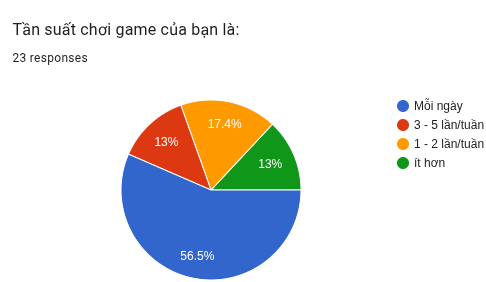
\includegraphics[width=.78\textwidth,height=.58\textheight,keepaspectratio]{frequency_game.png}\par
  \vfill
  \centering\textcolor{mutuxOrange}{\textbf{86,9\% có tần suất chơi hàng tuần: gaming là một hành vi lặp lại.}}
\end{frame}

\begin{frame}{Khảo sát 2/3: Gear đã từng mua}{Chuột, bàn phím và tai nghe là ba nhóm phổ biến nhất}
  \centering
  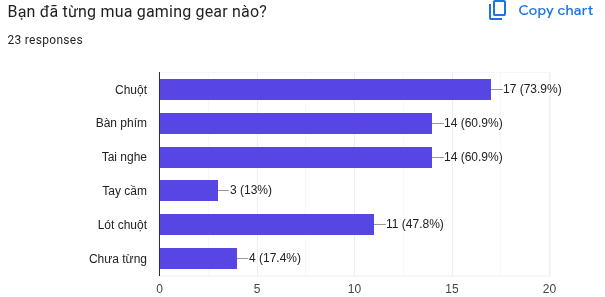
\includegraphics[width=.82\textwidth,height=.58\textheight,keepaspectratio]{gaming_gear_bought.png}\par
  \vfill
  \centering\textcolor{mutuxOrange}{\textbf{19/23 người đã từng mua gear: thị trường không cần giáo dục từ đầu.}}
\end{frame}

\begin{frame}{Khảo sát 3/3: Mức độ quan tâm thuê thử}{18/23 người hứng thú hoặc sẵn sàng cân nhắc}
  \centering
  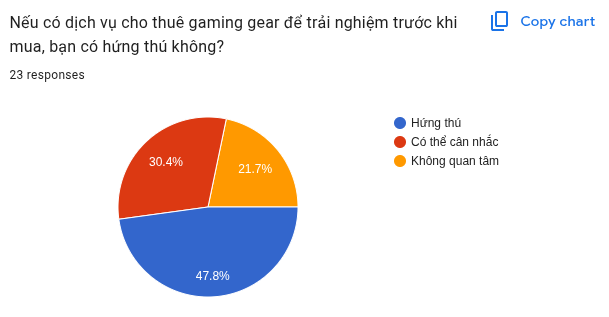
\includegraphics[width=.78\textwidth,height=.58\textheight,keepaspectratio]{Maybe_rent.png}\par
  \vfill
  \centering\textcolor{mutuxOrange}{\textbf{78,2\% mở với đề xuất thuê để trải nghiệm trước khi mua.}}
\end{frame}

\begin{frame}{Cách nhóm thí điểm cơ hội này}{Bắt đầu quanh ĐHQG-HCM với phạm vi đủ nhỏ để đo được}
  \vspace{.8em}
  \begin{columns}[T,onlytextwidth]
    \column{.30\textwidth}
      \cookiekicker{Đối tác}\par\vspace{.45em}
      3--5 shop neo và câu lạc bộ sinh viên quanh ĐHQG-HCM.
    \column{.30\textwidth}
      \cookiekicker{Kênh thử nghiệm}\par\vspace{.45em}
      Giải đấu sinh viên, cộng đồng gaming và social content.
    \column{.30\textwidth}
      \cookiekicker{Điều cần đo}\par\vspace{.45em}
      Tỷ lệ tạo đơn, hoàn tất, tranh chấp và tái thuê.
  \end{columns}
\end{frame}

\section{Sản phẩm và dịch vụ}

\begin{frame}{Sản phẩm / dịch vụ của nhóm}{Marketplace hai chiều cho gaming gear}
  \begin{columns}[T,onlytextwidth]
    \column{.42\textwidth}
      \begin{block}{Người thuê}
        Tìm kiếm, lọc, chọn thời gian, đặt cọc, thanh toán và nhận gear tại nơi sử dụng.
      \end{block}
    \column{.42\textwidth}
      \begin{exampleblock}{Chủ gear / Shop}
        Đăng thiết bị, quản lý lịch, nhận đơn, theo dõi doanh thu và tiếp cận khách mua mới.
      \end{exampleblock}
  \end{columns}
  \vspace{.75em}
  \centering
  \begin{tikzpicture}[node distance=1.25cm]
    \node[cookie accent node,minimum width=2.3cm] (r) {Người thuê};
    \node[cookie node,minimum width=2.7cm,right=of r] (m) {Mutux};
    \node[cookie node,minimum width=2.6cm,right=of m] (l) {Chủ gear};
    \draw[cookie arrow] (r) -- (m);
    \draw[cookie arrow] (m) -- (l);
  \end{tikzpicture}
\end{frame}

\begin{frame}{Hành trình sử dụng}{Thuê thử trước, mua khi đã chắc}
  \centering
  \begin{tikzpicture}[node distance=7mm]
    \node[cookie accent node,minimum width=1.75cm] (a) {Khám phá};
    \node[cookie node,minimum width=1.75cm,right=of a] (b) {Đặt thuê};
    \node[cookie node,minimum width=1.75cm,right=of b] (c) {Dùng thật};
    \node[cookie node,minimum width=1.75cm,right=of c] (d) {Đánh giá};
    \node[cookie node,minimum width=2.15cm,right=of d] (e) {Mua / thuê lại};
    \foreach \x/\y in {a/b,b/c,c/d,d/e} \draw[cookie arrow] (\x) -- (\y);
  \end{tikzpicture}
  \vspace{1em}
  \begin{block}{Lớp tin cậy}
    KYC xác minh người dùng, hồ sơ thiết bị ghi nhận tình trạng, escrow giữ tiền và đánh giá tạo dữ liệu sau giao dịch.
  \end{block}
\end{frame}

\section{Khách hàng mục tiêu}

\begin{frame}{Khách hàng mục tiêu}{Hai phía của marketplace}
  \begin{columns}[T,onlytextwidth]
    \column{.46\textwidth}
      \begin{block}{Renter -- Người thuê}
        \begin{itemize}\small
          \item Học sinh, sinh viên
          \item Người đi làm, creator
          \item Game thủ bán chuyên
        \end{itemize}
      \end{block}
    \column{.46\textwidth}
      \begin{exampleblock}{Lender -- Người cho thuê}
        \begin{itemize}\small
          \item Shop gaming gear SME
          \item Chủ quán net/gaming center
          \item Cá nhân sưu tầm gear
        \end{itemize}
      \end{exampleblock}
  \end{columns}
  \vfill
\end{frame}

\begin{frame}{Nỗi đau chính}{Mỗi phía có một lý do để tham gia}
  \begin{columns}[T,onlytextwidth]
    \column{.46\textwidth}
      \begin{block}{Renter}
        \begin{itemize}\small
          \item \textbf{Sinh viên:} thiếu ngân sách, sợ mua nhầm.
          \item \textbf{Người đi làm:} cần thử lâu, ít thời gian.
          \item \textbf{Bán chuyên:} cần gear tốt, độ chính xác cao sử dụng trong thời gian ngắn.
        \end{itemize}
      \end{block}
    \column{.46\textwidth}
      \begin{exampleblock}{Lender}
        \begin{itemize}\small
          \item \textbf{Shop:} hàng demo khấu hao.
          \item \textbf{Quán net:} gear dự phòng bỏ trống.
          \item \textbf{Cá nhân:} sợ mất, tráo gear.
        \end{itemize}
      \end{exampleblock}
  \end{columns}
  \vfill
\end{frame}

% \begin{frame}{Khách hàng ưu tiên trong MVP}{Bắt đầu hẹp, tạo thanh khoản}
%   \begin{columns}[T,onlytextwidth]
%     \column{.46\textwidth}
%       \begin{block}{Renter}
%         \centering\large\textbf{Sinh viên/game thủ}\par
%         \begin{itemize}\small
%           \item Tập trung đông
%           \item Dễ tiếp cận
%           \item Lan truyền tốt
%         \end{itemize}
%       \end{block}
%     \column{.46\textwidth}
%       \begin{exampleblock}{Lender}
%         \centering\large\textbf{Shop gaming gear SME}\par
%         \begin{itemize}\small
%           \item Có gear mẫu đa dạng
%           \item Có quy trình bàn giao
%           \item Dễ chuyển đổi sang mua
%         \end{itemize}
%       \end{exampleblock}
%   \end{columns}
%   \vfill
%   \centering\textbf{MVP: Sinh viên \textrightarrow Shop SME}
\end{frame}

\section{Điểm khác biệt}

\begin{frame}{Sản phẩm khác biệt như thế nào?}{Mutux đưa trải nghiệm về đúng không gian của người dùng}
  \centering\small
  \begin{tabularx}{.9\textwidth}{@{}Xccc@{}}
    \toprule
    \textbf{Tiêu chí} & \textbf{Showroom} & \textbf{Tiệm net} & \textbf{Mutux} \\
    \midrule
    Dùng tại nhà nhiều ngày & -- & -- & \textbf{Có} \\
    Thuê riêng từng thiết bị & -- & Hạn chế & \textbf{Có} \\
    KYC, cọc và escrow & -- & -- & \textbf{Có} \\
    Đánh giá gắn với thiết bị & Hạn chế & -- & \textbf{Có} \\
    Cơ hội mua sau khi thử & Có & -- & \textbf{Có} \\
    \bottomrule
  \end{tabularx}
  \vspace{.65em}
  \begin{block}{Lợi thế tích lũy}
    Mỗi đơn thuê tạo thêm hồ sơ tình trạng và phản hồi thực tế, giúp marketplace đáng tin hơn theo thời gian.
  \end{block}
\end{frame}

\section{Tiếp cận thị trường}

\begin{frame}{Ba kênh tiếp cận thị trường}{Kiểm chứng thủ công trước, mở rộng sau}
  \vspace{1em}
  \begin{columns}[T,onlytextwidth]
    \column{.29\textwidth}
      \cookiekicker{Community}\par\vspace{.45em}
      CLB trường, Discord, Facebook group và buổi dùng thử.
    \column{.29\textwidth}
      \cookiekicker{Content}\par\vspace{.45em}
      TikTok, video so sánh và đánh giá gear trong tình huống thật.
    \column{.29\textwidth}
      \cookiekicker{Partnership}\par\vspace{.45em}
      Shop SME, phòng máy, gaming cafe và giải đấu sinh viên.
  \end{columns}
\end{frame}

\begin{frame}{Lộ trình 12 tháng}{Mỗi giai đoạn có một mục tiêu duy nhất}
  \vspace{1.4em}
  \centering
  \begin{tikzpicture}[x=1cm]
    \draw[cookieLine,line width=1pt] (0,0) -- (10.8,0);
    \foreach \x/\label/\detail in {1.2/1--2/kiểm chứng,4.0/3--4/tối ưu,6.9/5--6/mở rộng,9.8/12 tháng/scale theo KPI} {
      \fill[cookieAccent] (\x,0) circle[radius=2.2pt];
      \node[above=3mm,font=\small\bfseries] at (\x,0) {\label};
      \node[below=3mm,font=\scriptsize,text=cookieMuted] at (\x,0) {\detail};
    }
  \end{tikzpicture}
  \vfill
  \centering\textcolor{mutuxOrange}{\textbf{Chỉ mở rộng khi các chỉ số của giai đoạn trước đạt yêu cầu.}}
\end{frame}

\section{Mô hình kiếm tiền}

\begin{frame}{Doanh thu đến từ mỗi đơn thuê hoàn tất}{Năm đầu ưu tiên phí nền tảng, các nguồn thu khác mở rộng sau}
  \vspace{.8em}
  \begin{columns}[T,onlytextwidth]
    \column{.30\textwidth}
      \cookiekicker{Phí nền tảng}\par\vspace{.45em}
      Thu 30\% trên giá trị tiền thuê của giao dịch hoàn tất.
    \column{.30\textwidth}
      \cookiekicker{Hiển thị ưu tiên}\par\vspace{.45em}
      Shop trả phí để tiếp cận đúng nhu cầu đã được xác thực.
    \column{.30\textwidth}
      \cookiekicker{Hoa hồng mua sau thuê}\par\vspace{.45em}
      Nhận hoa hồng khi trải nghiệm chuyển thành quyết định mua.
  \end{columns}
  \vfill
  \centering\textbf{Đơn thuê hoàn tất} $\rightarrow$ \textbf{Doanh thu lặp lại} $\rightarrow$ \textbf{Dịch vụ giá trị cao}
\end{frame}

\begin{frame}{Dự phóng năm 1}{Tập trung vào lực kéo từ giao dịch thuê}
  \vspace{1.2em}
  \centering
  \metric{1,11 tỷ}{GMV năm 1}
  \metric{\textasciitilde340 triệu}{doanh thu năm 1}
  \metric{7.050}{đơn thuê mục tiêu}
  \vfill
  \centering\small\color{cookieMuted}
  Cơ sở: 30\% phí nền tảng trên đơn thuê; chưa tính doanh thu B2B chưa kiểm chứng.
\end{frame}

\begin{frame}{Doanh thu theo quý}{Tăng trưởng dồn về nửa sau của năm đầu}
  \vspace{1.4em}
  \centering
  \small
  \begin{tabularx}{.8\textwidth}{@{}Xrrrr@{}}
    \toprule
    & \textbf{Q1} & \textbf{Q2} & \textbf{Q3} & \textbf{Q4} \\
    \midrule
    Doanh thu (triệu VNĐ) & 14 & 29 & 86 & 212 \\
    \bottomrule
  \end{tabularx}
  \vfill
  \centering\textcolor{mutuxOrange}{\textbf{Nửa đầu năm để kiểm chứng, nửa sau để tăng tốc.}}
\end{frame}

\begin{frame}{Các chỉ số cần chứng minh trước khi scale}{Tăng trưởng chỉ có ý nghĩa khi cung, cầu và an toàn cùng được kiểm soát}
  \vspace{.8em}
  \begin{columns}[T,onlytextwidth]
    \column{.30\textwidth}
      \cookiekicker{Chi phí thu hút}\par\vspace{.45em}
      CAC dưới 60.000 VNĐ cho mỗi người thuê có đơn hoàn tất.
    \column{.30\textwidth}
      \cookiekicker{An toàn tài sản}\par\vspace{.45em}
      Tổn thất thiết bị dưới 1\% trên tổng số đơn.
    \column{.30\textwidth}
      \cookiekicker{Chất lượng vận hành}\par\vspace{.45em}
      Theo dõi KYC, hủy đơn, tranh chấp và tái thuê.
  \end{columns}
  \vfill
  \centering\Large\textcolor{mutuxBlue}{\textbf{Cung $+$ Cầu $+$ An toàn}}
\end{frame}

\section{Gọi vốn và sử dụng vốn}

\begin{frame}{300 triệu VNĐ Pre-Seed}{Khoản vốn để vượt qua giai đoạn cold-start}
  \vspace{1.2em}
  \centering
  \metric{300 triệu}{vốn cần gọi}
  \metric{231 triệu}{thiếu hụt lớn nhất ở Q3}
  \metric{+91 triệu}{dòng tiền hoạt động Q4}
  \metric{Q3 năm 2}{hòa vốn lũy kế}
  \vfill
  \centering\small\color{cookieMuted}
  231 triệu bù thiếu hụt tiền mặt năm 1; phần còn lại là bộ đệm vận hành và rủi ro.
\end{frame}

\begin{frame}{Sử dụng vốn để làm gì?}{Ưu tiên công nghệ lõi, tăng trưởng và vận hành}
  \vspace{.8em}
  \centering\small
  \begin{tabularx}{.88\textwidth}{@{}Xrr@{}}
    \toprule
    \textbf{Hạng mục} & \textbf{VNĐ} & \textbf{Tỷ lệ} \\
    \midrule
    Marketing và trợ giá đơn đầu & 90 triệu & 30,0\% \\
    Sản phẩm và hạ tầng & 80 triệu & 26,7\% \\
    Vận hành và nhân sự & 90 triệu & 30,0\% \\
    Pháp lý & 20 triệu & 6,7\% \\
    Dự phòng rủi ro & 20 triệu & 6,7\% \\
    \bottomrule
  \end{tabularx}
  \vfill
  \centering\small\color{cookieMuted}
  Trọng tâm kỹ thuật: eKYC, escrow, PayOS, ví, đối soát và xử lý tranh chấp.
\end{frame}

\begin{frame}{Giải ngân theo cột mốc}{Vốn được mở dần theo tiến độ kiểm chứng}
  \vspace{1em}
  \begin{columns}[T,onlytextwidth]
    \column{.21\textwidth}
      \cookiekicker{Q1 --- 120 triệu}\par\vspace{.4em}
      MVP, eKYC--escrow, pháp lý và khởi động cold-start.
    \column{.21\textwidth}
      \cookiekicker{Q2 --- 90 triệu}\par\vspace{.4em}
      Pilot, trợ giá đơn đầu, CSKH và đo CAC.
    \column{.21\textwidth}
      \cookiekicker{Q3 --- 60 triệu}\par\vspace{.4em}
      Mở rộng đối tác, sự kiện sinh viên và hạ tầng.
    \column{.21\textwidth}
      \cookiekicker{Q4 --- 30 triệu}\par\vspace{.4em}
      Thử nghiệm B2B, hiển thị ưu tiên và quỹ dự phòng.
  \end{columns}
\end{frame}

\begin{frame}{Điều kiện chuyển pha}{Ba chỉ số quyết định việc mở khoản giải ngân tiếp theo}
  \vspace{1.2em}
  \begin{columns}[T,onlytextwidth]
    \column{.30\textwidth}
      \cookiekicker{CAC}\par\vspace{.45em}
      Nhỏ hơn hoặc bằng 60.000 VNĐ mỗi người thuê có đơn hoàn tất.
    \column{.30\textwidth}
      \cookiekicker{Tổn thất thiết bị}\par\vspace{.45em}
      Duy trì dưới 1\% trên tổng số đơn thuê.
    \column{.30\textwidth}
      \cookiekicker{Hoàn tất \& tái thuê}\par\vspace{.45em}
      Hai tỷ lệ này phải cải thiện qua từng quý.
  \end{columns}
  \vfill
  \centering\textcolor{mutuxOrange}{\textbf{Không đạt chỉ số thì không mở pha tiếp theo.}}
\end{frame}

\section{Đội ngũ}

\begin{frame}{Đội ngũ thực hiện}{Năng lực kỹ thuật phù hợp với bài toán marketplace}
  \vspace{.6em}
  \small
  \begin{tabularx}{.9\textwidth}{@{}lXl@{}}
    \toprule
    \textbf{Thành viên} & \textbf{Năng lực} & \textbf{Vai trò} \\
    \midrule
    Trần Cao Vân & Web/app, ML, quản lý nhóm & PM / Frontend \\
    Lê Hồ Đan Anh & Phân tích nghiệp vụ, backend & BA / Backend \\
    Lưu Huy Minh Quang & Web, CI/CD, gaming gear & Product owner \\
    Lê Tuấn Lộc & Fullstack, API, thanh toán, cloud & Backend / Marketing \\
    Nguyễn Hồ Anh Quốc & Frontend, bảo mật, dữ liệu & Frontend / Finance \\
    \bottomrule
  \end{tabularx}
\end{frame}

\begin{frame}{Lợi thế và khoảng trống}{Nhóm biết mình mạnh ở đâu và cần bổ sung gì}
  \vspace{1.2em}
  \begin{columns}[T,onlytextwidth]
    \column{.46\textwidth}
      \begin{exampleblock}{Lợi thế}
        Kinh nghiệm đồ án phần mềm, hackathon và hoạt động sinh viên.
      \end{exampleblock}
    \column{.46\textwidth}
      \begin{block}{Cần bổ sung}
        Marketing, tài chính và pháp lý --- nhóm đang tìm cố vấn cho các mảng này.
      \end{block}
  \end{columns}
\end{frame}

\section{Prototype và minh chứng}

\begin{frame}{Kết quả prototype / demo}{Luồng MVP đã được thiết kế và trực quan hóa}
  \begin{columns}[T,onlytextwidth]
    \column{.31\textwidth}
      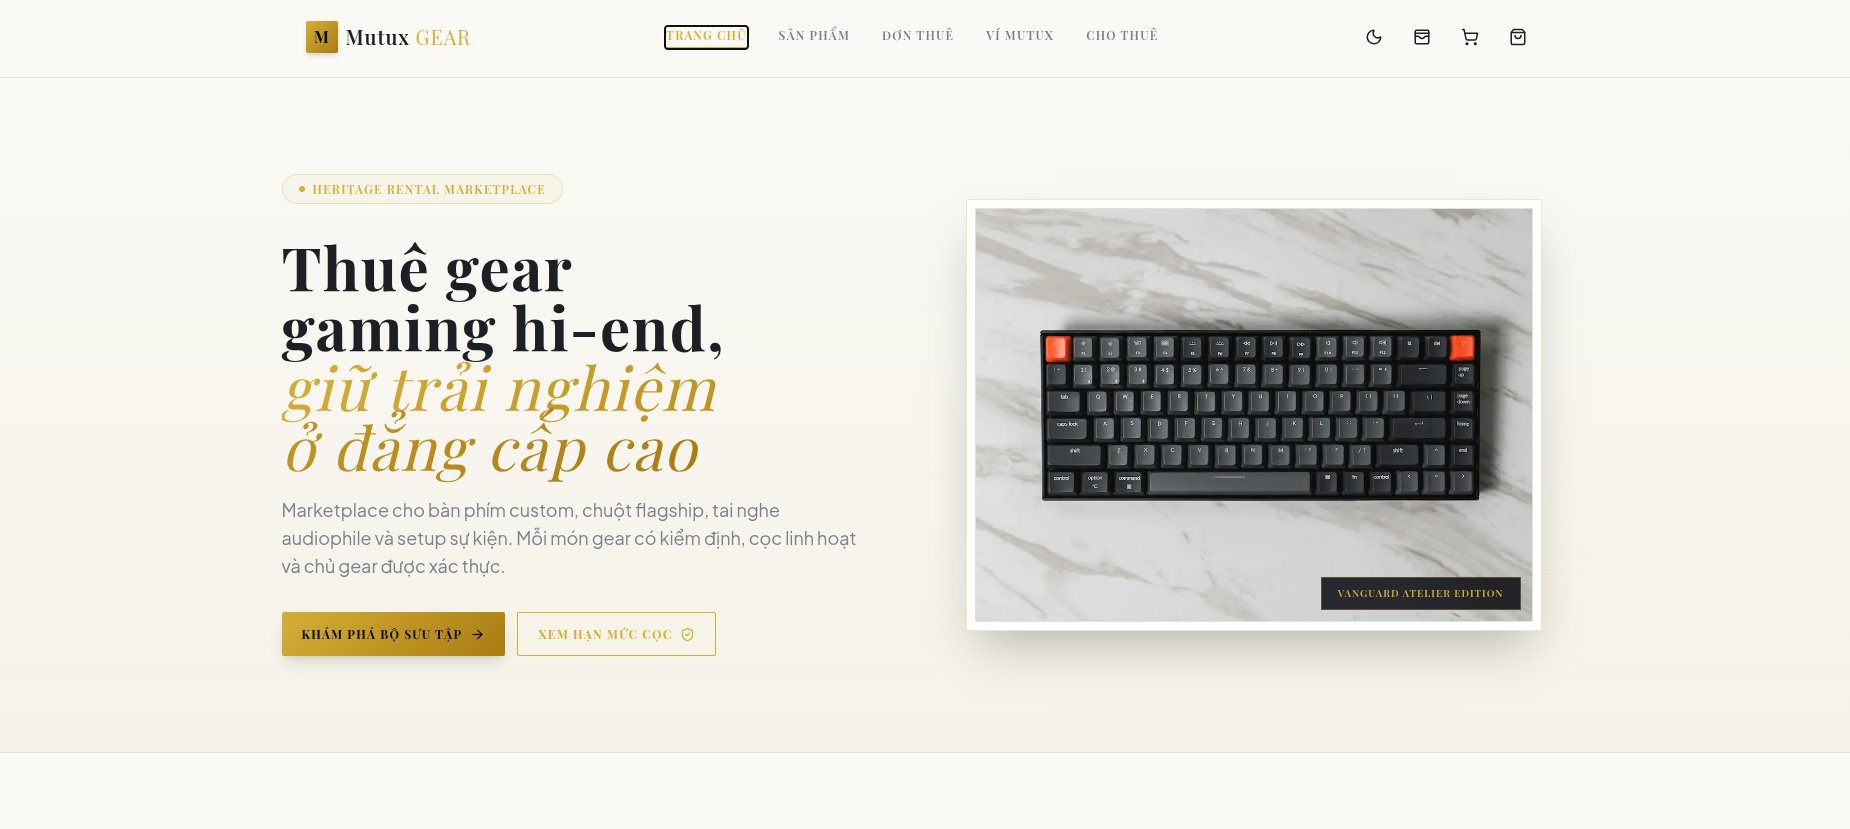
\includegraphics[width=\linewidth,height=.29\textheight,keepaspectratio]{frontpage1.png}\par
      \centering\scriptsize Landing page
      \vspace{.5em}
      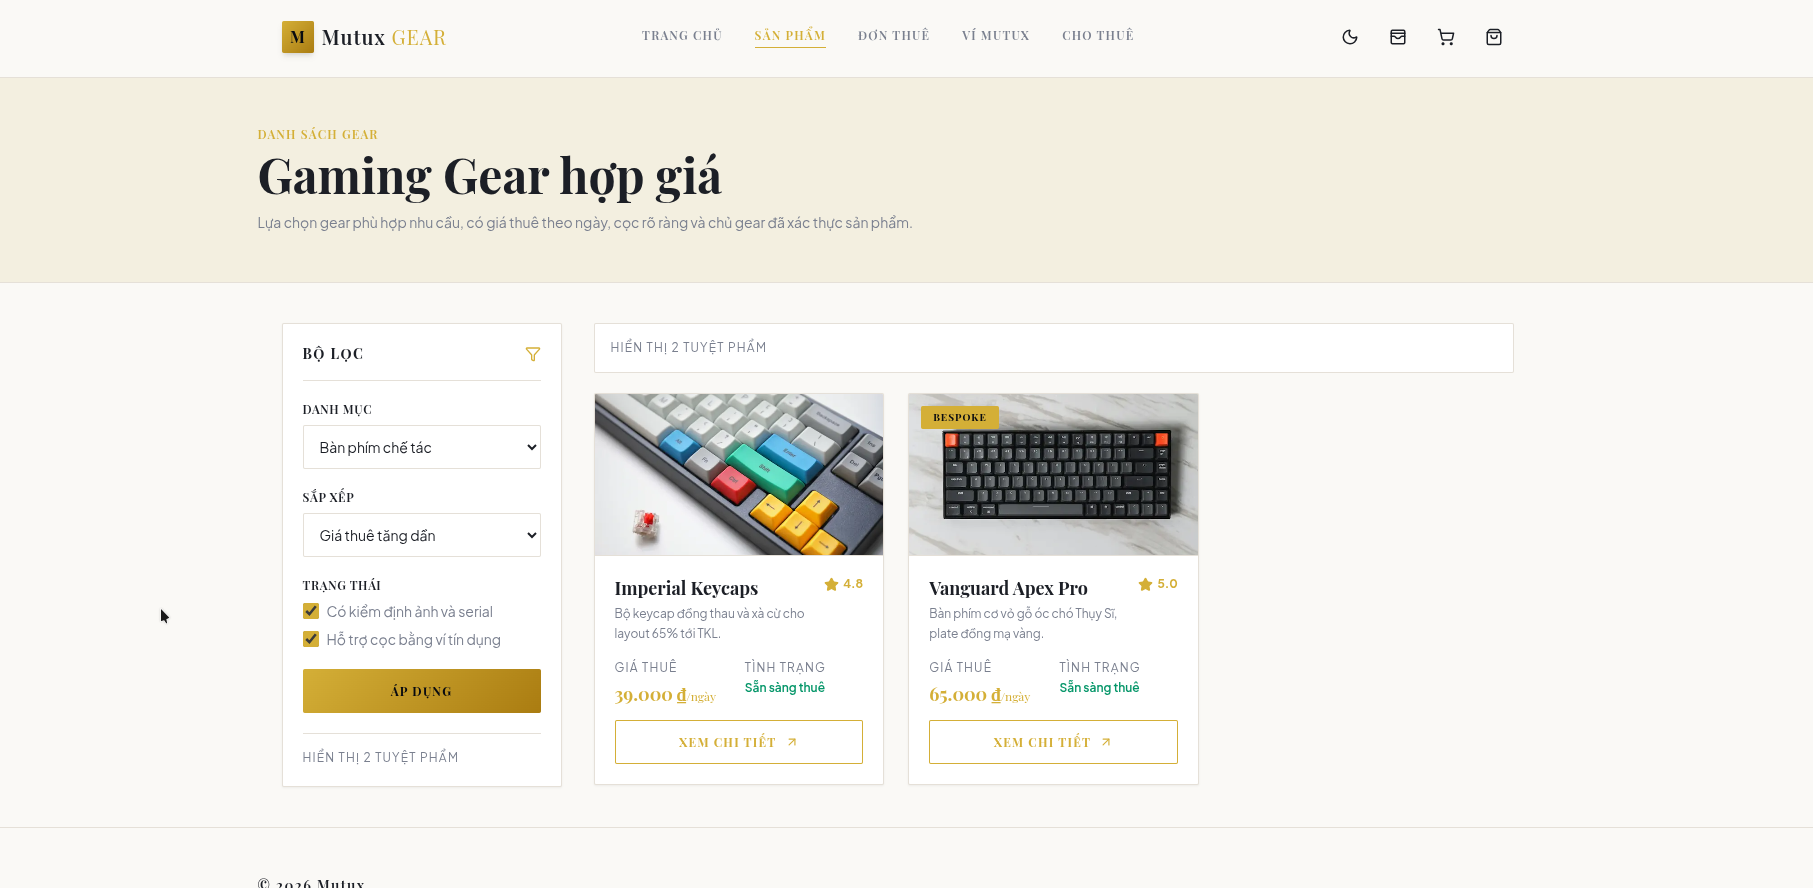
\includegraphics[width=\linewidth,height=.29\textheight,keepaspectratio]{listgear-filter.png}\par
      \centering\scriptsize Danh mục và bộ lọc
    \column{.31\textwidth}
      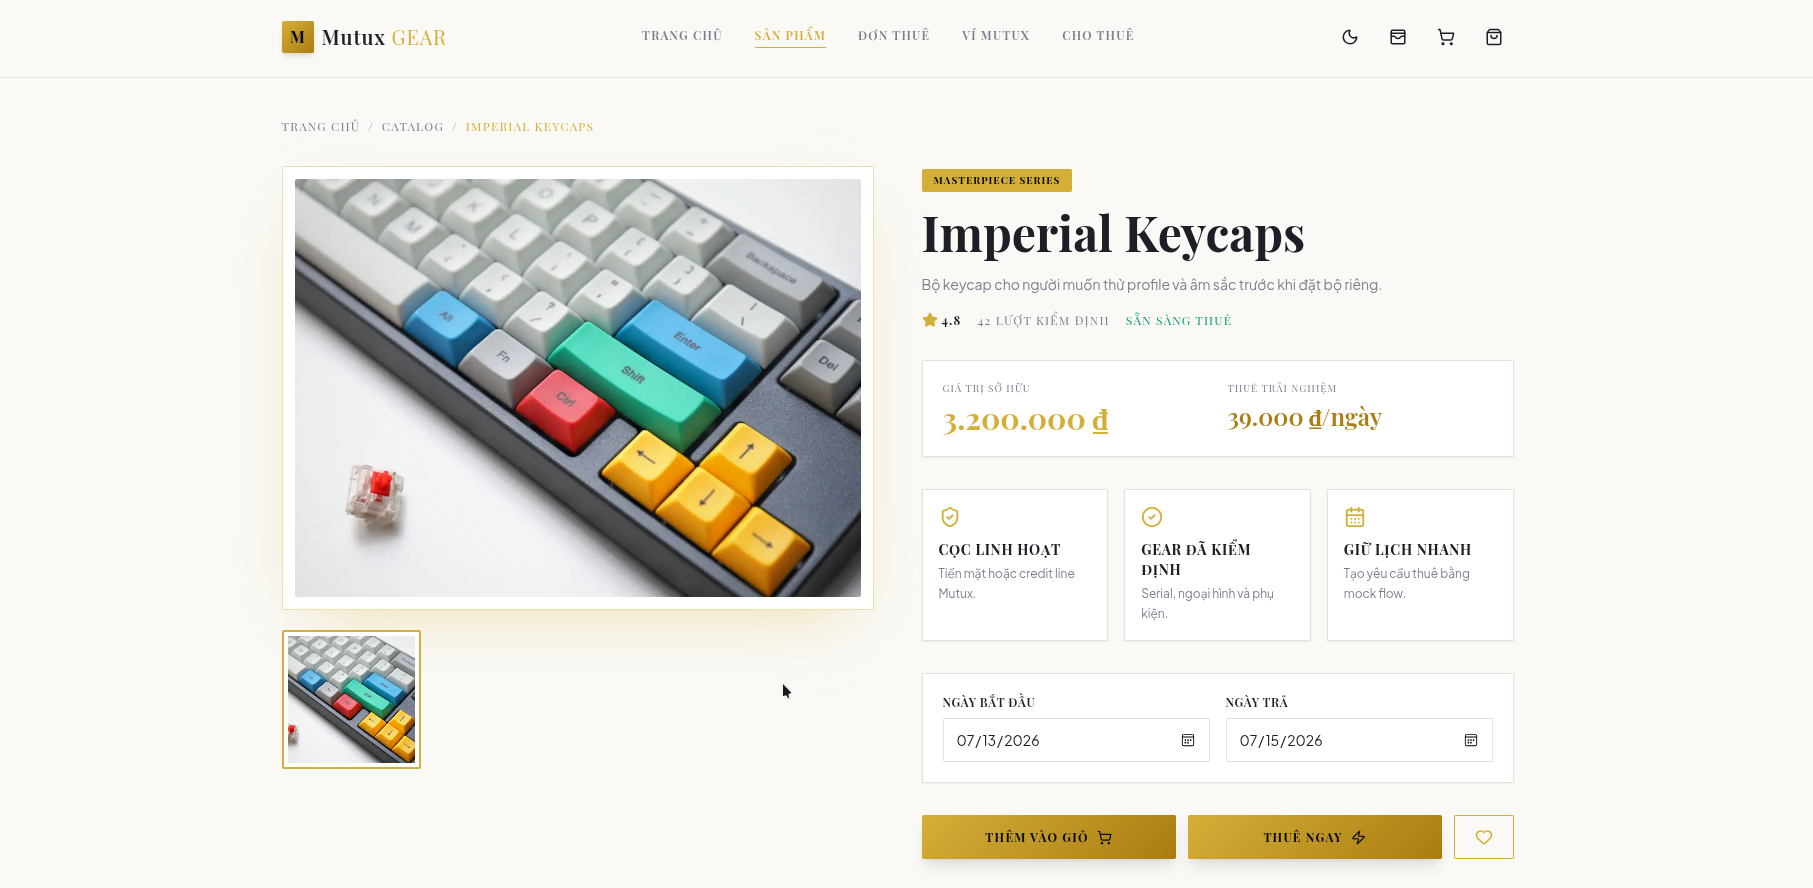
\includegraphics[width=\linewidth,height=.29\textheight,keepaspectratio]{detailgear.png}\par
      \centering\scriptsize Chi tiết và ngày thuê
      \vspace{.5em}
      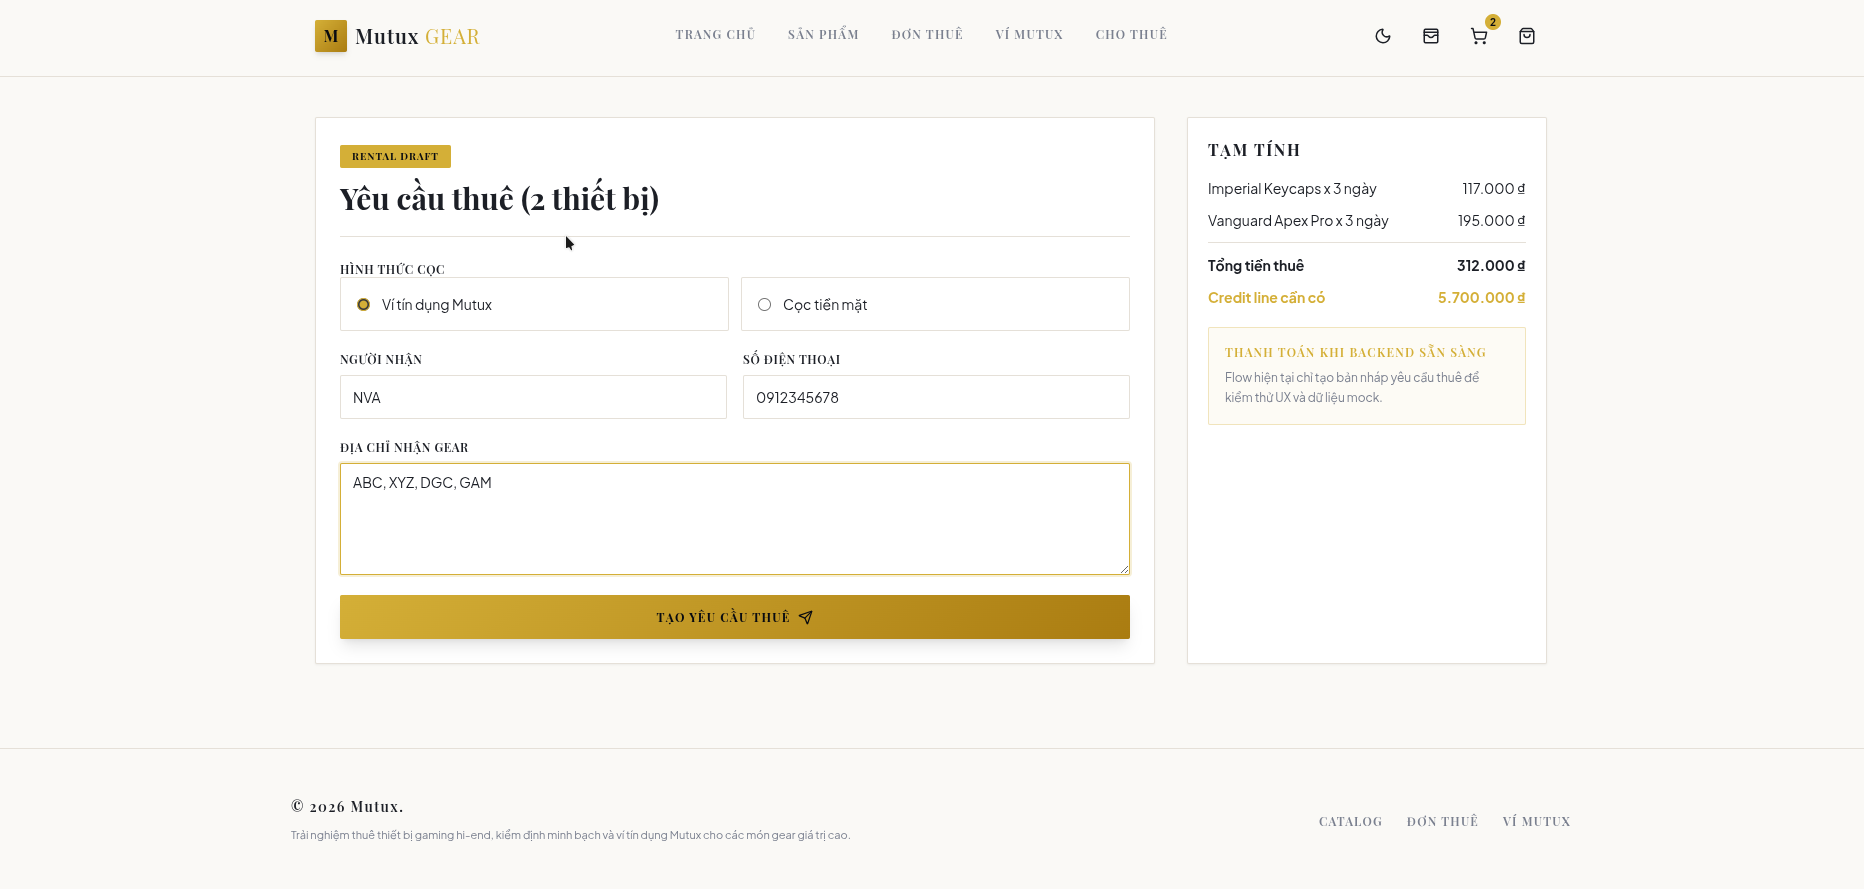
\includegraphics[width=\linewidth,height=.29\textheight,keepaspectratio]{payment.png}\par
      \centering\scriptsize Thanh toán và tiền cọc
    \column{.27\textwidth}
      \begin{block}{Luồng chính}
        Khám phá gear, chọn thời gian, tạo yêu cầu thuê, theo dõi ví và quản lý đơn hàng.
      \end{block}
      \cookiebadge{MVP UI}\par\vspace{.3em}\cookiebadge{Marketplace}
  \end{columns}
\end{frame}

\begin{frame}{Minh chứng triển khai và bước tiếp theo}{Từ prototype đến giao dịch thí điểm có kiểm soát}
  \begin{columns}[T,onlytextwidth]
    \column{.43\textwidth}
      \begin{exampleblock}{Đã có}
        Prototype giao diện, phân tích khách hàng, mô hình doanh thu, kế hoạch marketing, tài chính và codebase web đang phát triển.
      \end{exampleblock}
    \column{.43\textwidth}
      \begin{block}{Tiếp theo}
        Chọn 3--5 shop neo, chạy pilot quanh ĐHQG-HCM, hoàn thiện KYC--escrow và đo CAC, tỷ lệ hoàn tất, tranh chấp, tái thuê.
      \end{block}
  \end{columns}
  \vfill
  \centering\Large\textcolor{mutuxBlue}{\textbf{Trải nghiệm đúng. Quyết định chắc.}}
\end{frame}

\begin{frame}[plain,noframenumbering]
  \begin{tikzpicture}[remember picture,overlay]
    \fill[mutuxBlue] (current page.south west) rectangle (current page.north east);
    \node[anchor=west,text=white,text width=.68\paperwidth,align=left]
      at ($(current page.west)+(.105\paperwidth,.04\paperheight)$)
      {{\fontsize{29}{34}\selectfont\bfseries Cùng Mutux biến trải nghiệm\\thành quyết định đúng}\par\vspace{.65em}
       {\Large Thuê thử gear chuẩn gu, mua khi đã chắc.}};
    \draw[white,line width=1.4pt]
      ($(current page.west)+(.105\paperwidth,-.20\paperheight)$)
      -- ($(current page.west)+(.27\paperwidth,-.20\paperheight)$);
    \node[anchor=east,text=white!80,font=\small]
      at ($(current page.east)+(-.07\paperwidth,-.34\paperheight)$)
      {mutux.startup@gmail.com};
  \end{tikzpicture}
\end{frame}


\end{document}
